\documentclass[8pt,notitlepage,twocolumn]{report}

\usepackage{amsfonts}
\usepackage{amssymb}
\usepackage{amsthm}
\usepackage{amsmath,amscd}
\usepackage[all]{xy}
\usepackage{moreverb}
\usepackage{fancyhdr}
\usepackage{graphicx}


    \newtheorem{problem}{Problem}
    \newtheorem{theorem}{Theorem}[section]
    \newtheorem{lemma}[theorem]{Lemma}
    \newtheorem{proposition}[theorem]{Proposition}
    \newtheorem{corollary}[theorem]{Corollary}

    \newenvironment{solution}[1][Solution]{\begin{trivlist}
    \item[\hskip \labelsep {\bfseries #1}]}{\end{trivlist}}
    \newenvironment{definition}[1][Definition]{\begin{trivlist}
    \item[\hskip \labelsep {\bfseries #1}]}{\end{trivlist}}
    \newenvironment{example}[1][Example]{\begin{trivlist}
    \item[\hskip \labelsep {\bfseries #1}]}{\end{trivlist}}
    \newenvironment{remark}[1][Remark]{\begin{trivlist}
    \item[\hskip \labelsep {\bfseries #1}]}{\end{trivlist}}

  %  \newcommand{\qed}{\nobreak \ifvmode \relax \else
  %        \ifdim\lastskip<1.5em \hskip-\lastskip
  %        \hskip1.5em plus0em minus0.5em \fi \nobreak
  %        \vrule height0.75em width0.5em depth0.25em\fi}

    \renewcommand{\qedsymbol}{\textsquare}

\addtolength{\textwidth}{1in}
\addtolength{\hoffset}{-0.5in}
\addtolength{\textheight}{2in}
\addtolength{\voffset}{-0.3in}

\relpenalty=9999
\binoppenalty=9999

\newcommand{\PP}{\mathbb{P}}

\pagestyle{fancy}
%\fancyhead[CO,CE]{S.Chaichenets}
\fancyfoot[CO,CE]{S.Chaichenets}
\fancyfoot[RO, LE] {\thepage}


\begin{document}

\title{STAT 580 Stochastic Processes: HW 2}
\author{ S.\ Chaichenets }
\maketitle


%%%%%%%%%%%%%%%%%%%%%%%%%%%%%%%%%%%%%%%%%%%%

\begin{problem}
Markov chain with 
\small
\begin{equation}
P = 
\bordermatrix{
	& \mathbf{0} & \mathbf{1} & \mathbf{2} & \mathbf{3} & \mathbf{4} \cr
\mathbf{0} &  \frac{1}{2} & \frac{1}{2} & 0 & 0 & 0 \cr
\mathbf{1} &  \frac{1}{6} & \frac{5}{6} & 0 & 0 & 0 \cr
\mathbf{2} &  0 & 0 & \frac{3}{4} & \frac{1}{4} & 0 \cr
\mathbf{3} &  0 & 0 & \frac{1}{6} & \frac{5}{6} & 0 \cr
\mathbf{4} &  \frac{1}{5} & \frac{1}{5} & \frac{1}{5} & \frac{1}{5} & \frac{1}{5} \cr
}
\end{equation}
\normalsize

\SelectTips{cm}{}
\xymatrix{
	  	*+[o][F-]{0}	\ar@(dl,ul)[]^{\frac{1}{2}} \ar@/^/[r]^{\frac{1}{2}} %
	& 	*+[o][F-]{1} 	\ar@/^/[l]^{\frac{1}{6}} \ar@(ur,dr)[]^{\frac{5}{6}} %
	&  &  & 
	& 	*+[o][F-]{2}	\ar@(dl,ul)[]^{\frac{3}{4}} \ar@/^/[r]^{\frac{1}{4}} %
	& 	*+[o][F-]{3}	\ar@/^/[l]^{\frac{1}{6}} \ar@(ur,dr)[]^{\frac{5}{6}} %
	\\ %
	& & & 	*+[o][F-]{4} 	\ar@/^/[ulll]^{\frac{1}{5}} 	%
				\ar@/^/[ull]_{\frac{1}{5}} 	%
				\ar@/_/[urr]^{\frac{1}{5}} 	%
				\ar@/_/[urrr]_{\frac{1}{5}} 	%
				\ar@(ul,ur)^{\frac{1}{5}} & &
}

\end{problem}

\begin{solution}
It is trivial to verify that 
$\pi = \alpha (\frac{1}{4},\frac{3}{4},0,0,0) + (1-\alpha)(0,0,\frac{2}{5},\frac{3}{5},0) 
	\quad 0\leq\alpha\leq1$ 
is the general form of an invariant probability vector.
This means that the Ces\`aro mean is
\begin{equation}
  M = \bordermatrix{
	& \mathbf{0} & \mathbf{1} & \mathbf{2} & \mathbf{3} & \mathbf{4} 	\cr
\mathbf{0} & \frac{1}{4} & \frac{3}{4} & 0 & 0 & 0		\cr
\mathbf{1} & \frac{1}{4} & \frac{3}{4} & 0 & 0 & 0		\cr
\mathbf{2} & 0 & 0 & \frac{2}{5} & \frac{3}{5} & 0		\cr
\mathbf{3} & 0 & 0 & \frac{2}{5} & \frac{2}{5} & 0		\cr
\mathbf{4} & 0 & 0 & 0 & 0 & 0
}
=: (m_{ij})
\end{equation}
From this, we read off:\marginpar{{\bf 1(a)}}
$$
\mathbb{E}_0(T_0) = \frac{1}{m_{11}} = 4
$$
To determine $\mathbb{E}_1(T_0)$, we can consider only the transition matrix of the
$\{0,1\}$ communication class. Then `the $Q$ matrix' for state $0$ is simply $(5/6)$, 
hence\marginpar{{\bf(1(b)}}
$$
\mathbb{E}_1(T_0) = (1-\frac{5}{6})^{-1} = 6
$$
For $\mathbb{E}_5(T_1)$, We have to threat the recurrent class $\{2,3\}$ as part of the target set.
Then 
\scriptsize
$$
Q = \bordermatrix{
	& \mathbf{0} & \mathbf{4}	\cr
\mathbf{0} & \frac{1}{2} & 0		\cr
\mathbf{4} & \frac{1}{5} & \frac{1}{5}
} \qquad
(1-Q)^{-1} = \bordermatrix{
	& \mathbf{0} & \mathbf{4}	\cr
\mathbf{0} & 2 & 0		\cr
\mathbf{4} & \frac{1}{2} & \frac{5}{4}
}	
$$
\normalsize
Thus $$ \mathbb{E}_4(T_0) = 2 $$

Starting from the (transient) state 4, there is probability $\frac{4}{5}$ 
of escaping to either of the recurrent classes and never coming back. Therefore
$$
	\mathbb{P}_4(T_4<\infty) = \frac{1}{5}
$$

Again, from state 4, state 0 is only attainable we end up in its communicating class, 
the probability of which is clearly
$$
	\mathbb{P}_4(T_0<\infty) = \frac{1}{2}
$$
\qed
\end{solution}

\begin{problem}[waiting for patterns]
Fair coin tossed repeatedly; find the expected time to wait for pattern:

{\bf (i)} {HHHH}, {\bf (ii)} {THTH}
\end{problem}

\begin{solution}
{\bf HHHH}:
Introduce Markov chain with the following states:

	{\bf state~0}:{HHHH}
	{\bf state~1}:{XHHH\footnote{X is either of \{T,$\emptyset$\}}}
	{\bf state~2}:{XHH}
	{\bf state~3}:{XH}
	{\bf state~4}:{X}

The transition matrix for this chain is\footnote{
	I decided to do this question in slightly greater generality:
	$$\mathbb{P}({\rm H}) =: p = 1 - \mathbb{P}({\rm T}) =: 1-q $$
}
\begin{equation}
P = 
\bordermatrix{
		&\mathbf{4} 	& \mathbf{3} 	& \mathbf{2} 	& \mathbf{1} 	& \mathbf{0} 	\cr
\mathbf{4} 	& 	q 	& 	p 	& 	0 	& 	0 	& 0 		\cr
\mathbf{3} & q & 0 & p & 0 & 0		\cr
\mathbf{2} & q & 0 & 0 & p & 0		\cr
\mathbf{1} & q & 0 & 0 & 0 & p		\cr
\mathbf{0} & q & 0 & 0 & 0 & p
}
\end{equation}
Taking complement of the submatrix of transitions within the set $\{4,3,2,1\}$, 
we obtain\footnote{
	Using my latest fling with computer algebra software, 
	{\rm Maxima}, which goes way back to 1968 {\rm MIT}'s {\rm Macsyma} 
}
\begin{equation}
(I-Q)^{-1} = \frac{1}{p^4}
\bordermatrix{
		&\mathbf{4} 	& \mathbf{3} 	& \mathbf{2} 	& \mathbf{1} 	\cr
\mathbf{4} 	& 	1 	& 	p^1 	& 	p^2 	& 	p^3 	\cr
\mathbf{3} 	& 	p^3-1 	& 	p^1	& 	p^2 	& 	p^3 	\cr
\mathbf{2} 	& 	p^2-1	& 	p(p^2-1)& 	p^2 	& 	p^3	\cr
\mathbf{1} 	& 	p-1	& 	p(p-1) 	& 	p^2(p-1)& 	p^3	\cr
}
\end{equation}

Summing the top row, we obtain the expected time before hitting state $0$:
\begin{equation}
\mathbb{E}(T_0) = p^{-4} \frac{1-p^4}{q} 
\end{equation}
In case of a fair coin, $p=q=\frac{1}{2}$ and 
\marginpar{\bf{2(a)}}
$$ \mathbb{E}(T_0) = 2^4 \times \frac{1-\frac{1}{16}}{\frac{1}{2}} = 30$$
\marginpar{\small\bf{Aside}\normalsize}
Let us also mention the asymptotic behaviour as $p\to 0$, $p\to1$, $p=\frac{1}{2}(1+\epsilon)$:
\scriptsize
\begin{eqnarray*}
  p\to0^+ &\implies \mathbb{E}(T_0) &\approx \frac{p^{-4}}{q} \approx p^{-4} (1+p) \approx p^{-4} 	\\
  q\to0^+ &\implies \mathbb{E}(T_0) &= q^{-1} \left(-1+(\frac{1}{1-q})^4\right) 			\\
			& &= q^{-1} \left(-1 + 1 + 4q + \frac{4\times 5}{2}q^2 + O (q^3)\right) 	\\
			& &= 4 + 10q + O(q^2)								\\
  2p=1+\epsilon,2q=1-\epsilon &\implies \mathbb{E}(T_0) &= (2p)^{-4}\times2^4\frac{1-(2p)^4/2^4}{2q/2}\\
			& &= 2\frac{(1+\epsilon)^{-4}}{1-\epsilon}\left( 2^4-(1+\epsilon)^4 \right)	\\
			& &= 30 - 41\epsilon + O(\epsilon^2) 
\end{eqnarray*}
\normalsize
\qed
\end{solution}

\begin{solution}
{\bf THTH}:
\begin{itemize}
	\item[\quad state 0:] {THTH}
 	\item[state 1:] {TTHT or HTHT}
	\item[state 2:] {TTH or HTH}
	\item[state 3:] {TT,}
	\item[state 4:] {$\emptyset$ or $\emptyset\cdots$ H}
\end{itemize}
\begin{equation}
P = 
\bordermatrix{
		&\mathbf{4} 	& \mathbf{3} 	& \mathbf{2} 	& \mathbf{1} 	& \mathbf{0} 	\cr
\mathbf{4} 	& 	p 	& 	q 	& 	0 	& 	0 	& 0 		\cr
\mathbf{3} & 0 & q & p & 0 & 0		\cr
\mathbf{2} & p & 0 & 0 & q & 0		\cr
\mathbf{1} & 0 & q & 0 & 0 & p		\cr
\mathbf{0} & p & 0 & 0 & q & 0
}
\end{equation}
And
\tiny
\begin{equation}
(I-Q)^{-1} = 
\bordermatrix{
&\mathbf{4} 	& \mathbf{3} 	& \mathbf{2} 	& \mathbf{1} 	\cr
\mathbf{4} & -(p-2)/(p-1)^2 & -1/((p-1) p^2 & -1/((p-1)p) & 1/p 	\cr
\mathbf{3} & 1/(p-1)^2 	& -1/((p-1)p^2) & -1/((p-1)p) & 1/p		\cr
\mathbf{2} & 1/(p-1)^2	& -(p^2-p+1)/((p-1)p^2) & -1/((p-1)p) & 1/p	\cr
\mathbf{1} & -1/(p-1)	& 1/p^2		& 1/p	&1/p			
}
\end{equation}
\normalsize
In the case $p=q=\frac{1}{2}$, the top row sum is
$$
	\mathbb{E}_4(T_0) = 20
$$
\qed
\end{solution}

\begin{problem}[frog on a 3$\times$3 board]
\end{problem}

\begin{solution}
The transition matrix for the board is
\small
\begin{equation}
 P = 
 \bordermatrix{
	& \mathbf{11} & \mathbf{12} & \mathbf{13} & \mathbf{21} & \mathbf{22} & \mathbf{23} & \mathbf{31} & \mathbf{32} & \mathbf{33} \cr
\mathbf{11} & 	0	& \frac{1}{2}	& 0 	& \frac{1}{2} & 0 & 0 & 0 & 0 & 0	\cr
\mathbf{12} & \frac{1}{3} & 0 & \frac{1}{3} & 0 & \frac{1}{3} & 0 & 0 & 0 & 0		\cr
\mathbf{13} & 0 & \frac{1}{2} & 0 & 0 & 0 & \frac{1}{2} & 0 & 0 & 0			\cr
\mathbf{21} & \frac{1}{3} & 0 & 0 & 0 & \frac{1}{3} & 0 & \frac{1}{3} & 0 & 0		\cr
\mathbf{22} & 0 & \frac{1}{4} & 0 & \frac{1}{4} & 0 & \frac{1}{4} & 0 & \frac{1}{4} & 0 \cr
\mathbf{23} & 0 & 0 & \frac{1}{3} & 0 & \frac{1}{3} & 0 & 0 & 0 & \frac{1}{3}		\cr
\mathbf{31} & 0 & 0 & \frac{1}{2} & 0 & 0 & 0 & 0 & \frac{1}{2} & 0			\cr
\mathbf{32} & 0 & 0 & 0 & 0 & \frac{1}{3} & 0 & \frac{1}{3} & 0 & \frac{1}{3}		\cr
\mathbf{33} & 0 & 0 & 0 & 0 & 0 & \frac{1}{2} & 0 & \frac{1}{2} & 0
 }
\end{equation}
\normalsize
As usual, take $Q$ to be the upper $8\times8$ submatrix, and
\scriptsize
\begin{equation}
 (I-Q)^{-1} = 
 \bordermatrix{
& \mathbf{11} & \mathbf{12} & \mathbf{13} & \mathbf{21} & \mathbf{22} & \mathbf{23} & \mathbf{31} & \mathbf{32}\cr
\mathbf{11} & 3 & 3 & 3/2 & 3 & 3 & 3/2 & 3/2 & 3/2 		\cr
\mathbf{12} & 2 & 29/8 & 7/4 & 19/8 & 3 & 13/8 & 5/4 & 11/8 	\cr
\mathbf{13} & 3/2 & 21/8 & 5/2 & 15/8 & 5/2 & 15/8 & 1 & 9/8	\cr
\mathbf{21} & 2 & 19/8 & 5/4 & 29/8 & 3 & 11/8 & 7/4 & 13/8 	\cr
\mathbf{22} & 3/2 & 9/4 & 5/4 & 9/4 & 7/2 & 3/2 & 5/4 & 3/2	\cr
\mathbf{23} & 1   & 13/8 & 5/4 & 11/8 & 2 & 17/8 & 3/4 & 7/8	\cr
\mathbf{31} & 3/2 & 15/8 & 1   & 21/8 & 5/2 & 9/8 & 5/2 & 15/8	\cr
\mathbf{32} & 1   & 11/8 & 3/4 & 13/8 & 2 & 7/8 & 5/4 & 17/8
 }
\end{equation}
\normalsize
The expected length of a random walk from state $11$ to $33$ is the sum of the top row:\marginpar{{\tiny\bf 3(a)}}

$$ \mathbb{E}_{11}(33) = 18 $$
To verify this result, we run a computer simulation, using the code in Appendix \ref{q4code}.
In a series of runs with $2^{20}$ sample walks, we get $ \mu = 18 \pm .01 $
\marginpar{{\tiny\bf 4(a)}}
A histogram of the lengths distribution is given in figure \ref{qn4afig}. 
% We note that the distribution appears to be tail-heavy; a particularly intriguing feature is that
% $\sigma \approx 15$ for any sample size that we tried, between $2^5$ and $2^{25}$.
\begin{figure}[h]
 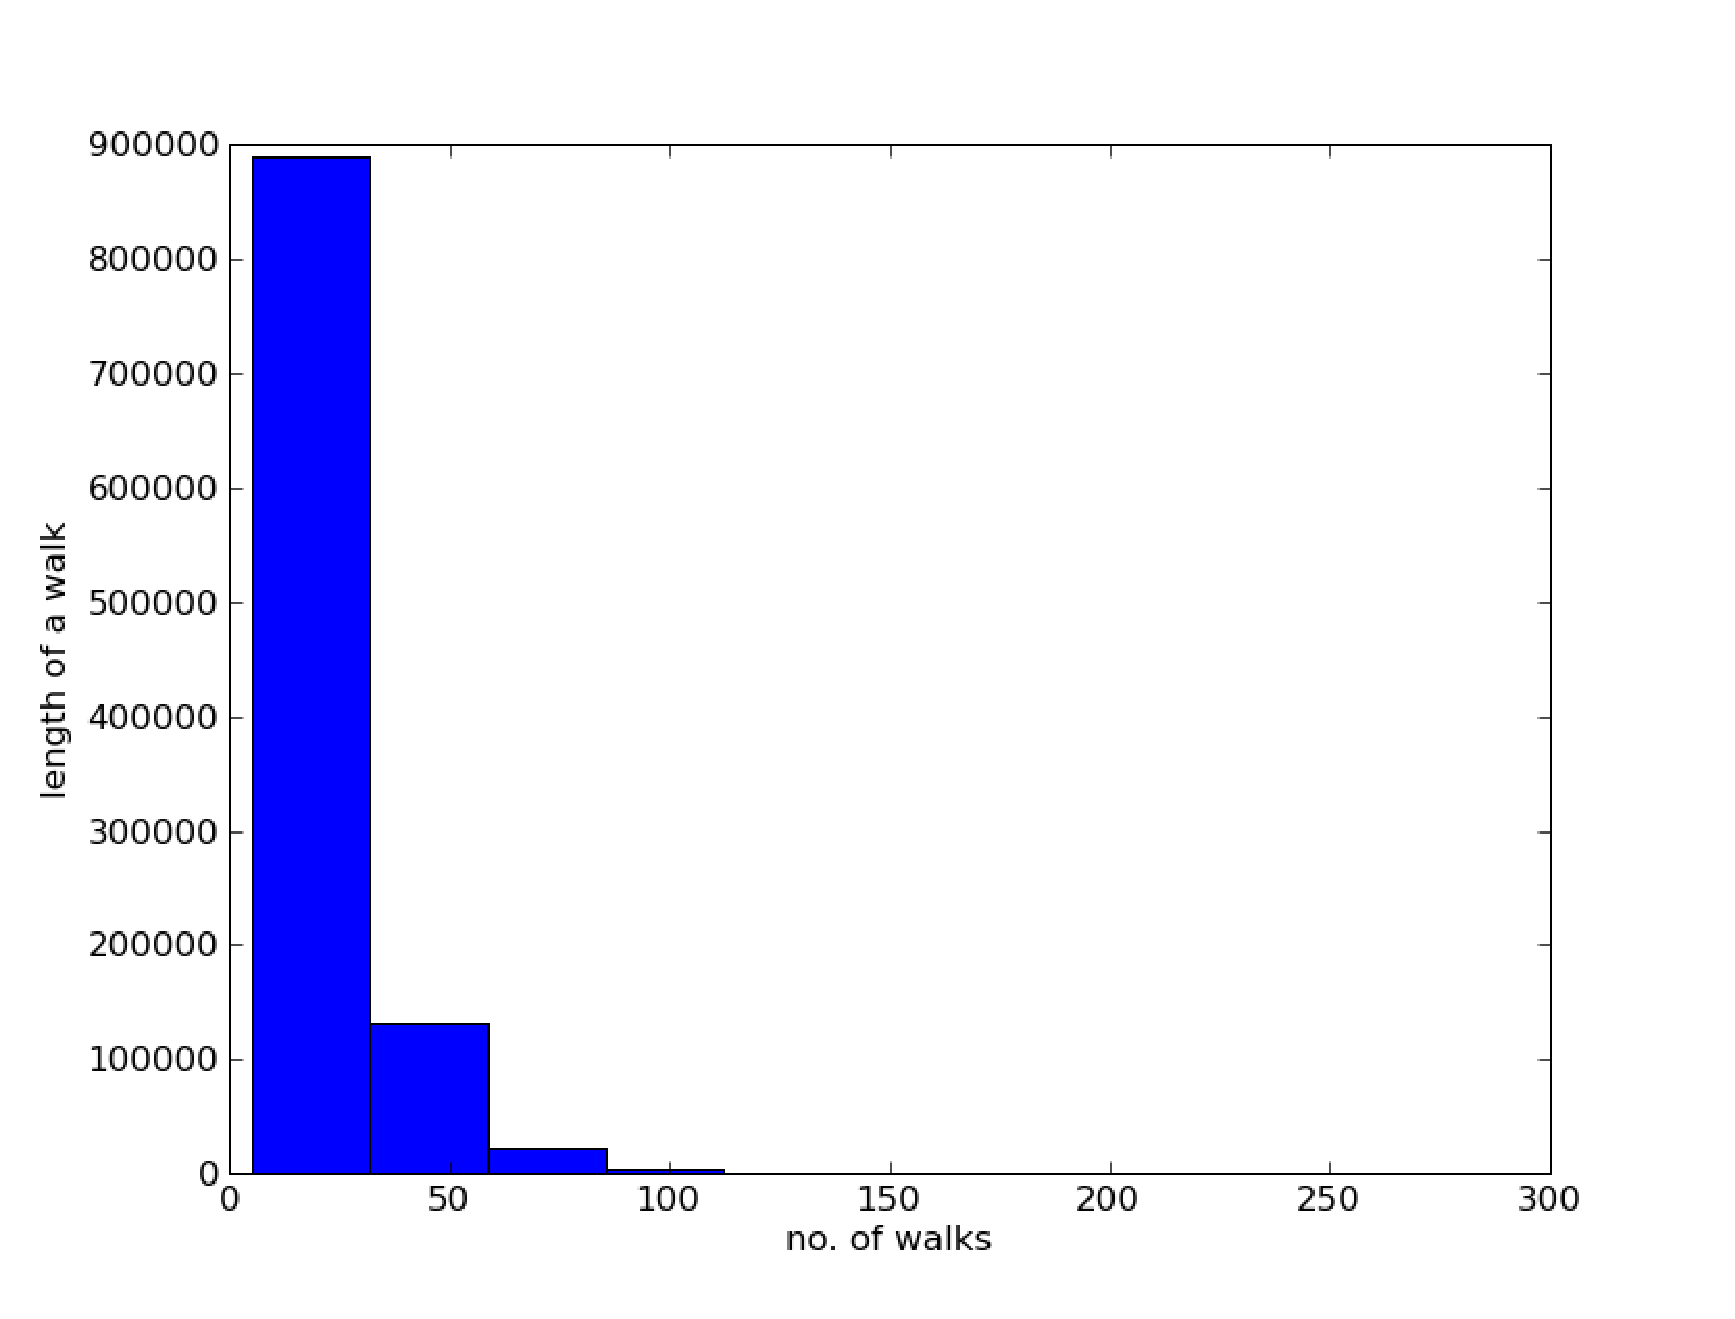
\includegraphics[height=.30\textheight]{hw2q4f1.eps}
 \caption{	lengths of random walks starting at 11 and terminating at 33. Sample size is $2^{20}$
   \label{qn4afig}
  }
\end{figure}
\qed
\end{solution}

\begin{problem}[Frog on $N\times N$ Board]
A simulation to estimate the hitting time of the $(NN)$ square, starting from $(11)$.
\end{problem}

\begin{solution}
We find that the mean length of a random walk grows as $\approx N^3$, 
as illustrated in figure \ref{hw2q4f2}
\begin{figure}[h]
 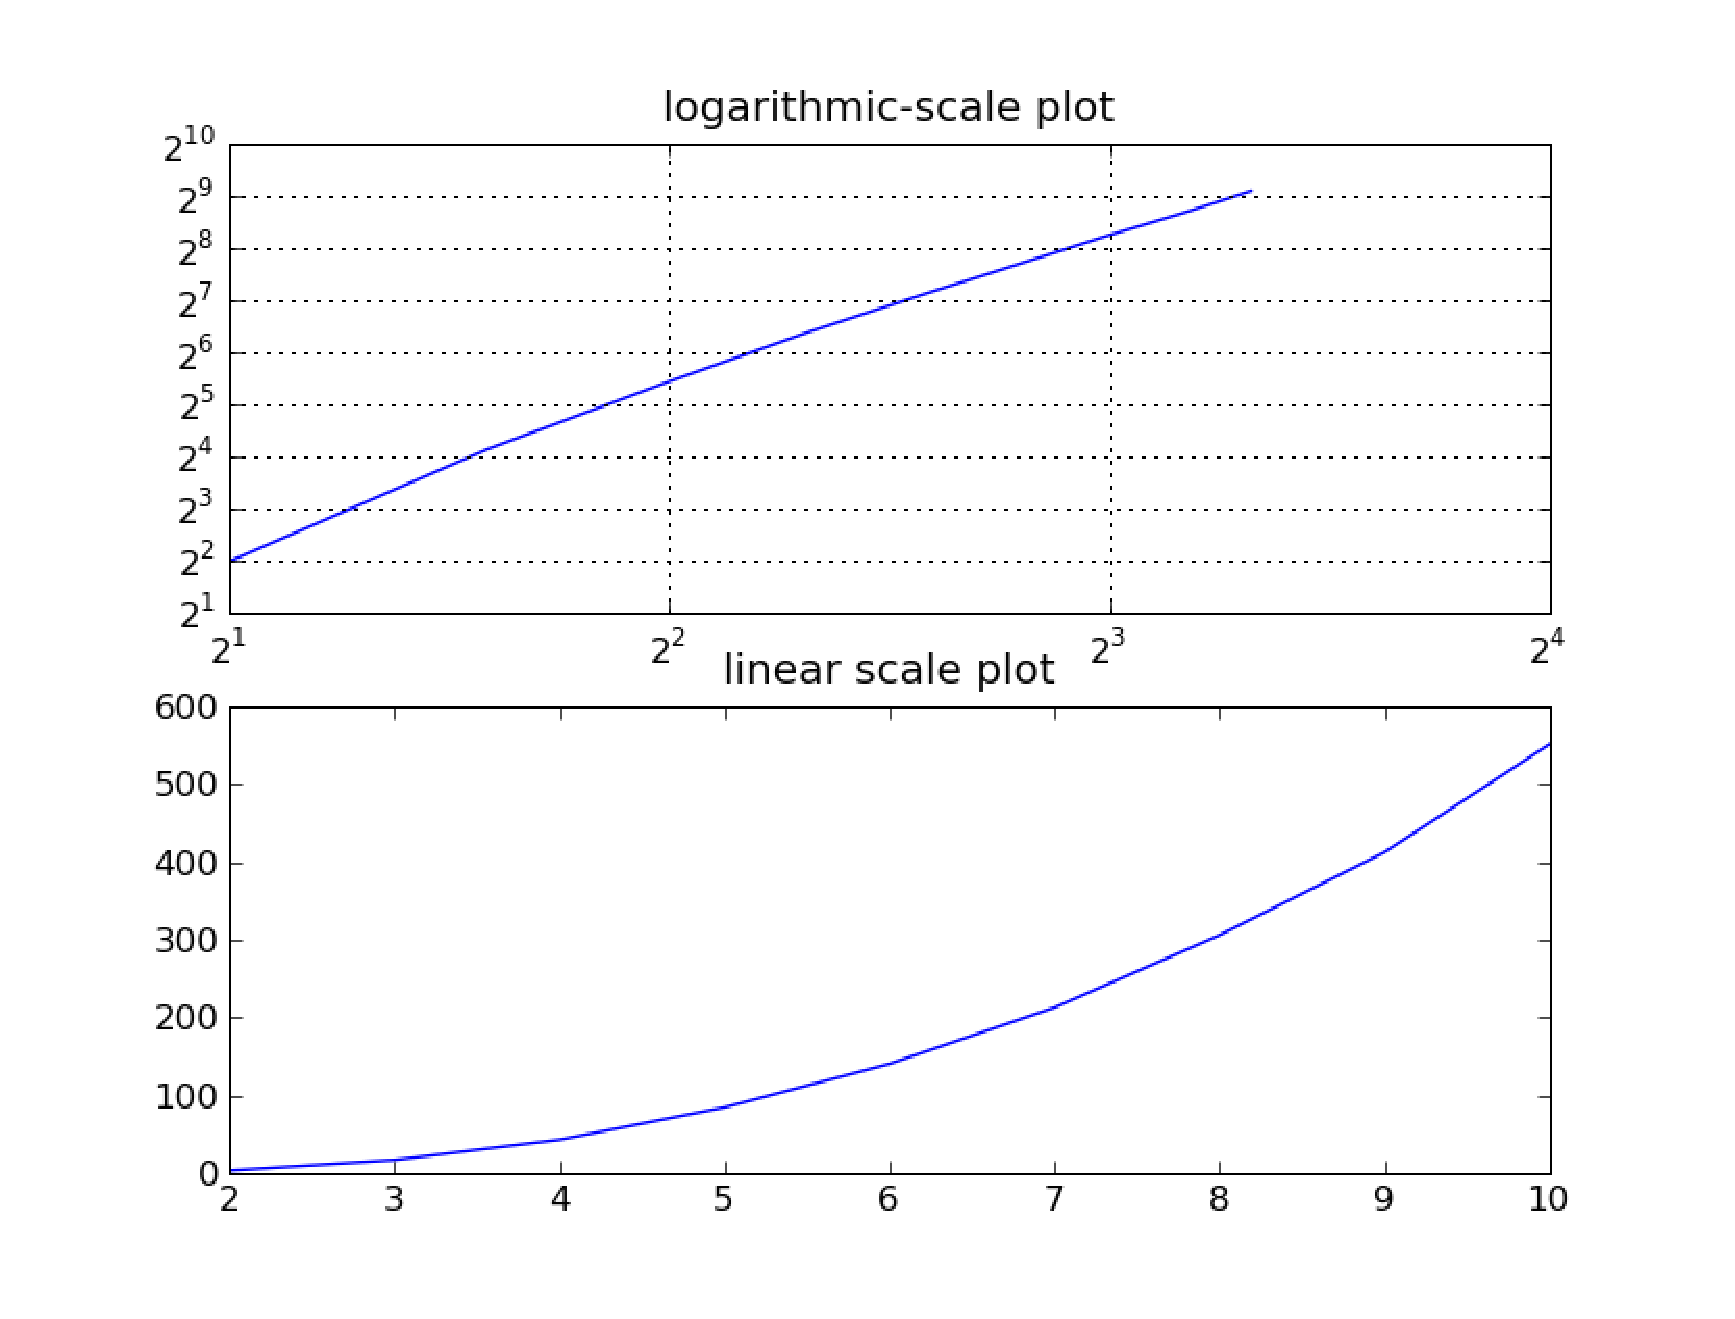
\includegraphics[height=.30\textheight]{nboard.eps}
 \caption{random walk length vs. board size.}
   \label{hw2q4f2}
\end{figure}
\qed
\end{solution}
\newpage
\appendix
\section{Code Listing: Random Walk on a $N\times N$ Board}
\label{q4code}
\verbatimtabinput[4]{hw2q4.py}

\end{document}
